\documentclass[dvipdfmx,fleqn]{beamer}
\usepackage{amsmath,amsthm,amssymb}
\usepackage{algorithm,algpseudocode}
\graphicspath{{./figure/}{./plot/}}
\makeatletter
\def\input@path{{./figure/}{./table/}}
\makeatother
\usepackage[
sorting=debug,
style=ieee,backend=bibtex,
texencoding=utf8,bibencoding=utf8,
dashed=false,
isbn=false,url=false,doi=false,
sorting=debug
]{biblatex}
\addbibresource{References.bib}
\AtBeginBibliography{}
\setbeamertemplate{bibliography item}[text]
\usetheme{IMELAB}
\usefonttheme[onlymath]{serif}

\usepackage{bxdpx-beamer}
\usepackage{pxjahyper}
\usepackage{verbatim}
%\usepackage[absolute,overlay]{textpos}

\renewcommand{\kanjifamilydefault}{\gtdefault}
\renewcommand{\familydefault}{\sfdefault}

% Theorem
\uselanguage{japanese}
\languagepath{japanese}
\deftranslation[to=japanese]{Theorem}{定理}
\deftranslation[to=japanese]{Lemma}{補題}
\deftranslation[to=japanese]{Example}{例}
\deftranslation[to=japanese]{Examples}{例}
\deftranslation[to=japanese]{Definition}{定義}
\deftranslation[to=japanese]{Definitions}{定義}
\deftranslation[to=japanese]{Problem}{問題}
\deftranslation[to=japanese]{Solution}{解}
\deftranslation[to=japanese]{Fact}{事実}
\deftranslation[to=japanese]{Proof}{証明}
\def\proofname{証明}

% Caption
\renewcommand{\figurename}{図}
\renewcommand{\tablename}{表}

% Beamer Misc.
\usepackage{appendixnumberbeamer}
\setbeamertemplate{navigation symbols}{}
\setbeamertemplate{frametitle continuation}[from second][(続き)]
%\setbeamertemplate{note page}[plain] % 基本これで
\setbeamertemplate{note page}{ % ちょこっとカスタマイズ
  \vspace{.5em}
  \insertslideintonotes{.30}
  \hfill
  {\tiny ページ\insertframenumber{}/\inserttotalframenumber}
  \noindent\rule{\textwidth}{.5pt}
  {\scriptsize\insertnote}
}
\setbeameroption{show notes}
%\setbeameroption{hide notes}
%\setbeameroption{show only notes}

\title[媒介中心性更新法]{辺操作時の最短経路の更新を利用する \\ 媒介中心性更新法}
\author[里谷]{里谷 佳紀}
\institute[情数工研]{情報数理工学研究室}
\date[研究発表会]{2019年度修士論文研究発表会 \\ 2020年2月12日}

\begin{document}

%\makeIMELABtitle
{
  \setbeamertemplate{footline}[imelab]
  \begin{frame}
    \titlepage
    \note[item]{ノートなのだ}
    \note[item]{情報数理工学研究室の里谷が}
    \note[item]{辺操作時の最短経路の更新を利用する媒介中心性更新法}
    \note[item]{という題目で発表します}
    \note[item]{よろしくおねがいします}
  \end{frame}
}

%\begin{frame}{概要}
%  \tableofcontents
%\end{frame}

\section{背景・目的}
\begin{frame}[t]{研究背景 -- 媒介中心性}
  \begin{itemize}
  \item \alert{媒介中心性}\footcite{05Freeman1977}:ネットワークのノードの重要度を測る.
  \item[] 例:鉄道網における駅
  \end{itemize}
  \begin{columns}
    \begin{column}{.4\textwidth}
      \begin{equation*}
        B_v=\sum_{s\neq v}\sum_{t\neq v,s}\frac{\sigma_{st}(v)}{\sigma_{st}},
      \end{equation*}
    \end{column}
    \begin{column}{.6\textwidth}
      \begin{itemize}
      \item $\sigma_{st}(v)$:$s$と$t$間の最短経路のうち\\$v$を通るものの数,
      \item $\sigma_{st}$:$s$と$t$間の最短経路の数.
      \end{itemize}
    \end{column}
  \end{columns}
  \medskip
  \begin{itemize}
  \item 媒介中心性の値が高い$\rightarrow$\alert{多くの最短経路が通る}ので重要
  \end{itemize}
  \vspace{-.5em}
  \begin{center}
    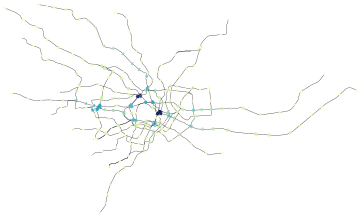
\includegraphics[width=.55\columnwidth]{tokyo-metro-betweenness.png}
  \end{center}
  \note[item]{まず研究背景として媒介中心性について説明します.}
  \note[item]{
    媒介中心性とはネットワークのノードの重要度を測る中心性と呼ばれる指標のひとつです.
  }
  \note[item]{媒介中心性の定義はこちらの式で与えられます.}
  \note[item]{
    ここで,$\sigma_{st}(v)$は$s$と$t$間の最短経路のうち$v$を通るものの数を,
    $\sigma_{st}$は$s$と$t$間の最短経路の数を表します.
  }
  \note[item]{
    あるノードの媒介中心性の値が高いと,そのノードの上に多くの最短経路が通っているので,
    重要であると言えます.
  }
  \note[item]{
    例えば,こちらにネットワークの図がありますが,媒介中心性の値が大きくなるほど色を濃くしています.
    ネットワークの中央付近のノードは最短経路が多く通っているため,濃く表示されています.
  }
\end{frame}

\begin{frame}{媒介中心性の計算例}
  \begin{columns}
    \begin{column}{.6\textwidth}
      頂点$v$の媒介中心性の値$B_v$は
      \begin{flalign*}
        B_v&=\sum_{s\neq v}\sum_{t\neq s,v}\frac{\sigma_{st}(v)}{\sigma_{st}}\\
        &=\frac{\sigma_{wx}(v)}{\sigma_{wx}}+\frac{\sigma_{wy}(v)}{\sigma_{wy}}
        +\frac{\sigma_{wz}(v)}{\sigma_{wz}}\\
        &+\frac{\sigma_{xy}(v)}{\sigma_{xy}}+\frac{\sigma_{xz}(v)}{\sigma_{xz}}
        +\frac{\sigma_{yz}(v)}{\sigma_{yz}}+\cdots\\
        &=\frac{0}{1}+\frac{0}{1}+\frac{1}{1}+\frac{0}{1}+\frac{2}{2}+\frac{1}{1}\cdots\\
        &=6.
      \end{flalign*}
      同様に,$B_w=B_y=2,\:B_x=B_z=0$.
    \end{column}
    \begin{column}{.39\textwidth}
      \centering
      \def\svgwidth{.9\linewidth}
      \input{graph-bc.pdf_tex}
    \end{column}
  \end{columns}
  \medskip
  計算量:\alert{$\mathcal{O}(|V|^3)$}
  \note[item]{ここで定義に従った媒介中心性の計算の例を示します.}
  \note[item]{右に示したグラフの$v$の媒介中心性は,このように計算されます.}
  \note[item]{
    ここで,定義に従った方法で全ての頂点の媒介中心性の値を計算したときの計算量について考えます.
  }
  \note[item]{
    総和記号の赤枠の部分から,和は頂点数$|V|$の二乗だけ繰り返されます.
    そのため,全ての頂点の媒介中心性の値の計算の計算量は$|V|$の三乗オーダです.
  }
  \note[item]{
    これでは,頂点数の増加とともに計算時間が膨大になり,巨大なネットワークの解析は困難です.
  }
\end{frame}

\begin{frame}{Brandesの定理}
  \begin{itemize}\small
  \item ペア依存度 $\delta_{st}(v)=\sigma_{st}(v)/\sigma_{st}$
  \item 依存度
    $\delta_{s\bullet}(v)=\sum_{t\neq s,v}\sigma_{st}(v)/\sigma_{st}$
  \item 媒介中心性
    $B_v=\sum_{s\neq v}\colorlet{oldcolor}{.}\usebeamercolor[fg]{alerted text}\fbox{$\color{oldcolor}\sum_{t\neq s,v}\sigma_{st}(v)/\sigma_{st}$}\color{oldcolor}=\sum_{s\neq v}\delta_{s\bullet}(v)$
  \item $\delta_{s\bullet}(v)$を高速に計算したい
  \end{itemize}
  \begin{theorem}[Brandes \footcite{06Brandes2001}]\rm
    \label{th:implicit-dependency}
    グラフ$G=(V,E)$の異なる頂点$s,v$について,頂点$v$の$s$に対する依存度$\delta_{s\bullet}(v)$は次式を満たす.
    \begin{equation*}
      \delta_{s\bullet}(v)=\sum_{(v,w)\in E_s}\frac{\sigma_{sv}}{\sigma_{sw}}(1+\delta_{s\bullet}(w)).
    \end{equation*}
    ただし,$E_s$は$s$から各頂点への最短経路の辺集合である.
  \end{theorem}
  \begin{flushright}
    \alert{次で例を説明}
  \end{flushright}
  \note[item]{
    媒介中心性の値を高速に計算するため,Brandesは依存度と呼ばれる値を高速に計算しました.
  }
  \note[item]{
    依存度とは,$\sigma_{st}(v)/\sigma_{st}$を$t$について総和を取ったものです.
  }
  \note[item]{
    依存度の定義を使うと,媒介中心性の定義のこの部分が依存度に置き換わり,
    依存度を$s$について総和を取ったものを計算することで計算できます.
  }
  \note[item]{
    ここで依存度を高速に計算するため,Brandesは次の定理を示しました.
    この定理は,$s$に対する$v$の依存度は最短経路上で$v$の一つ後の頂点$w$の依存度から計算
    出来ることを示しています.
  }
  \note[item]{この定理を用いた計算例を次に示します.}
\end{frame}

\begin{frame}{Brandesのアルゴリズム}
  \begin{columns}
    \begin{column}{.49\textwidth}
      右図において
      \begin{equation*}\small
        \begin{aligned}
          \delta_{s\bullet}(v)&=\frac{\sigma_{sv}}{\sigma_{sw_1}}(1+\delta_{s\bullet}(w_1)) \\
          &+\frac{\sigma_{sv}}{\sigma_{sw_2}}(1+\delta_{s\bullet}(w_2)) \\
          &+\frac{\sigma_{sv}}{\sigma_{sw_3}}(1+\delta_{s\bullet}(w_3))
        \end{aligned}
      \end{equation*}
    \end{column}
    \begin{column}{.49\textwidth}
      \centering
      \def\svgwidth{.9\columnwidth}
      \input{implicit-dependency.pdf_tex}
    \end{column}
  \end{columns}
  \medskip
  \begin{enumerate}
  \item $s$からの最短経路$E_s$を計算
  \item 最短距離の降順に頂点を走査($w$とする)
  \item $(v,w)$が最短経路に含まれるような$v$に対して
  \item[] $\delta_{s\bullet}(v)\gets\delta_{s\bullet}(v)+\colorlet{oldcolor}{.}\usebeamercolor[fg]{alerted text}\fbox{$\color{oldcolor}\sigma_{sv}/\sigma_{sw}(1+\delta_{s\bullet}(w))$}\color{oldcolor}$
  \end{enumerate}
  計算量:\alert{$\mathcal{O}(|V|^2\log |V|+|V||E|)$}
  \note[item]{ここでBrandesの定理を使った依存度の計算の例を示します.}
  \note[item]{こちらの図に示した,頂点$s$からの最短経路で説明します.}
  \note[item]{$s$に対する$v$の依存度は,定理からこの式で計算できます.}
  \note[item]{ここで,最短経路の上で$v$の後継は$w$であることに注意します.}
  \note[item]{
    Brandesのアルゴリズムの手順を簡単に説明すると,こちらになります.
    まず$s$からの最短経路を計算します.
    その後,$s$から遠い順に頂点$w$を走査し,$w$の先行$v$に対して,この式で
    $v$の依存度を更新します.
  }
  \note[item]{
    Brandesのアルゴリズムで全ての頂点の媒介中心性を計算するときの計算量はこれで,
    疎なネットワークに対してある程度高速に媒介中心性を計算できます.
  }
\end{frame}

\begin{frame}{時変ネットワークの媒介中心性}
  \begin{columns}
    \begin{column}{.5\textwidth}
      \begin{itemize}
      \item 現実のネットワークは変化する
      \item[] \alert{時変ネットワーク}\cite{18Holme2012}
      \item[] 例:フォロー,道路の建設
      \item 時変ネットワークの媒介中心性計算
      \item[] 媒介中心性が変化する頂点は少ない
      \item[] 影響を受ける部分のみを効率的に計算したい
      \end{itemize}
    \end{column}
    \begin{column}{.5\textwidth}
      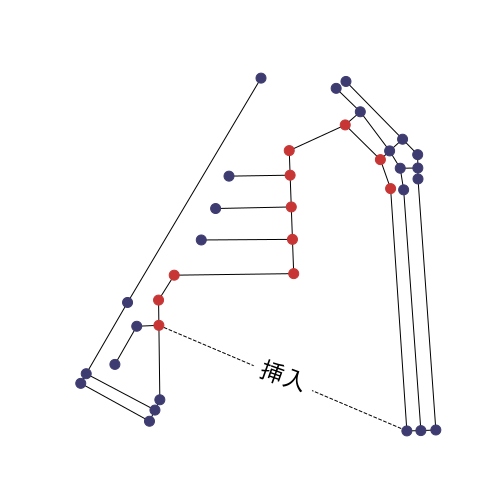
\includegraphics[width=.9\columnwidth]{road-sta.pdf}
    \end{column}
  \end{columns}
  \hypercite{18Holme2012}
  \note[item]{
    先ほど説明したBrandesのアルゴリズムは,ネットワークにノードやリンクが追加されない,
    時不変ネットワークに対して媒介中心性の値を計算します.
  }
  \note[item]{
    しかし現実のネットワークは,例えばSNSでのフォローや道路の建設などによって,
    その形が絶えず変化する時変ネットワークです.
  }
  \note[item]{
    このようなネットワークに対しては,変化の差分にあたる部分のみを計算し,
    媒介中心性の値を更新することで,
    Brandesのアルゴリズムを初めから適用するよりも高速に計算できると期待できます.
  }
  \note[item]{
    例えば,このネットワークにこのリンクを追加した場合,追加によって媒介中心性の値が
    変化するノードは赤く示したこれらのノードです.
  }
\end{frame}

\begin{frame}{関連研究}
  時変ネットワークの媒介中心性更新法
  \begin{itemize}\small
  \item Minimum union cycleを更新\cite{19Lee2012,20Singh2015}
  \item Hypergraph sketch\cite{17Yoshida2014}を更新する\cite{21Hayashi2015},
  \item 近似法を応用\cite{22Bergamini2015a,23Bergamini2015b}
  \item \alert{最短経路と共に媒介中心性を更新}
  \end{itemize}
  \begin{center}
    \scriptsize
    \begin{tabular}{lll}
      \hline
      アルゴリズム & 最短経路更新アルゴリズム & 辺の操作 \\ \hline
      Kasら\cite{25Kas2013} & RamalingamとReps\cite{24Ramalingam1996} & 挿入 \\ \hline
      Nasreら\cite{27Nasre2014a} & Kargerら\cite{26Karger1993} & 挿入 \\ \hline
      Nasreら\cite{29Nasre2014b} & DemetrescuとItaliano\cite{28Demetrescu2003} & 削除 \\ \hline
      Pontecorviら\cite{30Pontecorvi2015} & DemetrescuとItaliano\cite{28Demetrescu2003} & 挿入/削除 \\ \hline
      Bergaminiら\cite{31Bergamini2017} & RamalingamとReps\cite{24Ramalingam1996} & 挿入 \\ \hline
      \alert{本研究} & \alert{RamalingamとReps}\cite{24Ramalingam1996} & \alert{削除} \\ \hline
    \end{tabular}
  \end{center}
  \begin{block}{研究目的}
    \small
    RamalingamとRepsに基づく最短経路更新法を利用する \\
    辺削除時の媒介中心性更新法の提案と評価
  \end{block}
  \note[item]{
    そのため現在まで時変ネットワークの媒介中心性を更新する方法がいくつか提案されてきました.
  }
  \note[item]{
    Minimum union cycleやHypergraph sketchといった,専用のデータ構造を利用する方法や,
  }
  \note[item]{
    時不変ネットワークでも用いられた近似法を時変ネットワークに適用した方法の他に,
  }
  \note[item]{
    最短経路を保持し,媒介中心性と共に更新する方法もいくつか提案されてきました.
  }
  \note[item]{
    その中でも,RamalingamとRepsの最短経路更新アルゴリズムに基づく,
    辺削除時の媒介中心性更新法はこれまで提案されていませんでした.
  }
  \note[item]{
    そこで,この研究は,RamalingamとRepsの最短経路更新アルゴリズムに基づく,
    辺削除時の媒介中心性更新法の提案と評価を目的とします.
  }
\end{frame}
  
\section{提案アルゴリズム}
\begin{frame}[allowframebreaks]{提案アルゴリズム}
  記号について
  \begin{itemize}\small
    \item 辺$(u,v)$が削除されたと考える
    \item 記号$'$:削除後であることを表す(例:$G'$)
    \item $S(t)$:辺削除によって$t$への最短経路が変化する頂点の集合
    \item $T(s)$:辺削除によって$s$からの最短経路が変化する頂点の集合
    \item $\Delta_{s\bullet}(x)=\sum_{t\in T(s)}\delta_{st}(x)$:削除の影響を受けるペア依存度の総和\footcite{31Bergamini2017}
  \end{itemize}
  アルゴリズムの大まかな流れ
  \begin{algorithmic}\footnotesize
    \ForAll{$s\in S(v)$}
    \State $\textproc{DecreaseBetweenness}(s)$
    \Comment{\alert{$B_x$を$\sum_{s\neq x}\Delta_{s\bullet}(x)$だけ減少}}
    \State $\textproc{UpdateSSSP}(s)$
    \Comment{\alert{$d_{st}$と$\sigma_{st}$を更新}}
    \State $\textproc{IncreaseBetweenness}(s)$
    \Comment{$B_x$を$\sum_{s\neq x}\Delta'_{s\bullet}(x)$だけ増加}
    \EndFor
    \ForAll{$t\in T(u)$}
    \State $\textproc{UpdateSTSP}(t)$
    \Comment{$d_{st}$と$\sigma_{st}$を更新}
    \EndFor
  \end{algorithmic}
  \note[item]{以降,本研究で提案するアルゴリズムについて説明します.}
  \note[item]{グラフから辺$(u,v)$が削除されたと考えます.}
  \note[item]{
    削除後の諸量にプライム記号をつけて,それが削除後であることを明示します.
    例えば,削除後のグラフ$G$は$G'$で表します.
  }
  \note[item]{
    $S(t)$と$T(s)$はそれぞれ辺削除によって$t$への,および$s$からの最短経路が変化する頂点の集合とします.
    $S(t)$と$T(s)$の具体的な内容はあとで示します.
  }
  \note[item]{
    さらに$\Delta_{s\bullet}(x)$をこの通り定義します.
    これは削除の影響を受けるペア依存度$\delta_{st}(x)$の総和です.
  }
  \note[item]{
    アルゴリズムの大まかな流れは以下です.
    初めに$x\in V$に対する$\Delta_{s\bullet}(x)$を求めて,媒介中心性の値$B_x$から減算します.
    次に,各$t\in V$の$d_{st}$および$\sigma_{st}$を更新します.
    さらに,$x\in V$に対する$\Delta'_{s\bullet}(x)$を求めて,減算された媒介中心性の値$B''_s$に加算します.
  }
\end{frame}

\begin{frame}{影響を受ける頂点}
  $T(x)$と$S(x)$の具体的な内容を求める
  \begin{lemma}
    頂点$s,t$に対して,$E_{st}'\neq E_{st}$であるための必要十分条件は$d_{su}+l_{uv}+d_{vt}=d_{st}$を満たすことである.
  \end{lemma}
  \begin{columns}[T]
    \begin{column}{0.60\textwidth}
      \begin{itemize}
      \item $E_{st}'\neq E_{st}$ならば,$(u,v)$は最短経路の上にある
      \item すると,$d_{su}+l_{uv}+d_{vt}=d_{st}$が成り立つ
      \end{itemize}
    \end{column}
    \begin{column}{0.38\textwidth}
      \centering
      \def\svgwidth{.9\columnwidth}
      \input{condition-affection.pdf_tex}
    \end{column}
  \end{columns}
  \begin{itemize}
  \item $T(x)=\{t\,|\,d_{xt}=d_{xu}+l_{uv}+d_{vt}\}$
  \item $S(x)=\{s\,|\,d_{sx}=d_{su}+l_{uv}+d_{vx}\}$
  \end{itemize}
  両方とも,\alert{深さ優先探索}で計算可能
  \note[item]{ここで$S(x)$と$T(x)$の具体的な内容を求めます.}
  \note[item]{削除によって最短経路が変化する頂点ペアの条件について,こちらの補題を示しました.}
  \note[item]{
    読み上げますと,頂点$s,t$に対して,$E_{st}'\neq E_{st}$であるための
    必要十分条件は$d_{su}+l_{uv}+d_{vt}=d_{st}$を満たすことです.
  }
  \note[item]{
    その根拠は,最短経路が変化するならば,削除される辺$(u,v)$は最短経路の上にあり,
    すると,$d_{su}+l_{uv}+d_{vt}=d_{st}$が成り立つためです.
  }
  \note[item]{
    この補題によって,$S(x)$と$T(x)$の具体的な内容をこちらの通りに定義できます.
  }
  \note[item]{
    実際に内容を求めるには,削除される辺に接続する頂点$v$または$v$を視点として,
    深さ優先探索によって求められます.
  }
\end{frame}

\begin{frame}{$\Delta_{s\bullet}(x)$を求めるアルゴリズム}
  \begin{theorem}[Bergamini et al.\cite{31Bergamini2017}]\small
    任意の$s\in S(v)$と$x\in V$について,次式が成り立つ.
    \begin{equation*}
      \Delta_{s\bullet}(x)
      =\sum_{y\in\mathcal{S}_{G_s}(x)\cap T(s)}\frac{\sigma_{sx}}{\sigma_{sy}}(1+\Delta_{s\bullet}(y))
      +\sum_{y\in\mathcal{S}_{G_s}(x)\setminus T(s)}\frac{\sigma_{sx}}{\sigma_{sy}}\Delta_{s\bullet}(y)
    \end{equation*}
  \end{theorem}
  \begin{columns}
    \begin{column}{.49\textwidth}
      \begin{itemize}
      \item Brandesのアルゴリズムと同様に$s$から遠い順に走査する
      \item ただし,$s$と$t\in T(s)$の最短経路の間にある頂点のみを走査する
      \item $T(s)$に含まれているかどうかで加算する値は異なる
      \end{itemize}
    \end{column}
    \begin{column}{.49\textwidth}
      \centering
      \def\svgwidth{.9\columnwidth}
      \input{calculate-affected-delta.pdf_tex}
    \end{column}
  \end{columns}
  $\Delta'_{s\bullet}(x)$も同様に計算可能
  \note[item]{
    次は影響を受ける頂点のペア依存度の総和である$\Delta_{s\bullet}(x)$を求める
    方法について説明します.
  }
  \note[item]{
    $\Delta_{s\bullet}(x)$について,この式が成り立つことが知られています.
    この式は,影響を受ける頂点の,$x$についてのペア依存度の総和は,
    最短経路上で$x$の後継の頂点についてのペア依存度の総和から求められることを示しています.
  }
  \note[item]{
    この式を利用して$\Delta_{s\bullet}(x)$を求めるには,
    Brandesのアルゴリズムと同様に,$s$から遠い順に走査します.
  }
  \note[item]{
    ただし,Brandesのアルゴリズムでは全頂点を走査したのに対し,
    この方法では,影響を受ける頂点と,$s$とそれらの最短経路上にある頂点のみを走査します.
  }
  \note[item]{$\Delta'_{s\bullet}(x)$も同様に計算できます.}
\end{frame}

\begin{frame}{辺削除時の最短経路更新法(Ramalingam and Reps\footcite{24Ramalingam1996})}
  \begin{itemize}
  \item 更新後の距離の昇順に計算する必要がある
  \item[] しかしそのような並びは\alert{自明ではない}
  \item RamalingamとRepsの方法に基づき正しい順序で最短経路を更新する
  \end{itemize}
  \begin{columns}
    \begin{column}{.60\textwidth}
      \begin{enumerate}
      \item $x\in T(s)$のうち,$y\notin T(s)$を先行にもつ$x$はすぐに更新可能
      \item その距離と最短経路数はそれぞれ
        \begin{equation*}
          \begin{aligned}
            d'_{sx}&=\min\{d_{sx}+l_{xy}|y\in\mathcal{P}(x)\setminus T(s)\} \\
            \sigma'_{sx}&=\sum_{y\in \mathcal{P}_{G_s}(x)}\sigma_{sy}
          \end{aligned}
        \end{equation*}
      \item 以降,更新が完了した頂点から広げるように距離と最短経路数を更新
      \end{enumerate}
    \end{column}
    \begin{column}{.39\textwidth}
      \centering
      \def\svgwidth{.95\columnwidth}
      \input{updating-sssp.pdf_tex}
    \end{column}
  \end{columns}
  \note[item]{ここで,RamalingamとRepsに基づく変削除時の最短経路更新法について説明します.}
  \note[item]{
    RamalingamとRepsの方法ではDijkstramのアルゴリズムと同様に,
    削除に影響される頂点集合$T(s)$の各要素を,更新後の距離の昇順に走査する必要があります.
  }
  \note[item]{
    しかし,RamalingamとRepsの方法で知られている通り,
    $T(s)$の各要素を昇順に走査することは自明ではなく,計算時に判断する必要があります.
  }
  \note[item]{
    そこで提案手法では以下のアイディアで正しい順序で走査し,最短経路を更新します.
  }
  \note[item]{
    まず,影響を受ける頂点$x$のうち,影響を受けない頂点を先行にもつものは
    この式で削除後の$s$からの距離と最短経路数を更新できます.
  }
  \note[item]{
    あとは,Dijkstraのアルゴリズムの要領で更新が完了した頂点から広げるように
    $s$からの距離と最短経路数を更新します.
  }
\end{frame}

\section{性能評価}
\begin{frame}{時間計算量の評価}
  \begin{itemize}\small
    \item 媒介中心性を増減させるアルゴリズムの時間計算量
    \begin{equation*}
      \mathcal{O}\left(\sum_{s\in S(v)}\|\tau(s)\|+|\tau(s)|\log|\tau(s)|+\|\tau'(s)\|+|\tau'(s)|\log|\tau'(s)|\right)
    \end{equation*}
  \item[] $\tau(s),\,\tau'(s)$:アルゴリズムが走査した頂点の集合
  \item[] \alert{$S(v)=\tau(s)=\tau'(s)=V$}のときBrandesのアルゴリズムの計算量と同じ
    \item 最短経路を更新するアルゴリズムの時間計算量
    \begin{equation*}
      \mathcal{O}\left(\sum_{s\in S(v)}\|T(s)\|\log|T(s)|+\sum_{t\in T(u)}\|S(t)\|\log|S(t)|\right)
    \end{equation*}
  \item[] \alert{$S(v)=T(u)=V$}のときDijkstraのアルゴリズムの計算量と同じ
  \item 通常は$V$より小さい$\rightarrow$\alert{高速に動作}
  \end{itemize}
  \note[item]{以降,提案したアルゴリズムの性能を評価します.}
  \note[item]{まず,時間計算量を既存のものと比較します.}
  \note[item]{
    媒介中心性を増減させるアルゴリズムの時間計算量はこちらです.
    この計算量は,影響を受ける頂点の集合$S(v)$とアルゴリズムが走査した頂点の集合
    $\tau(s)$および$\tau'(s)$が頂点集合$V$と一致するとき,
    Brandesのアルゴリズムと同じ計算量になります.
  }
  \note[item]{
    最短経路を更新するアルゴリズムの時間計算量はこちらです.
    この計算量は,影響を受ける頂点の集合$S(v)$と$T(u)$が頂点集合$V$と一致するとき,
    Dijkstraのアルゴリズムと同じ計算量になります.
  }
  \note[item]{
    これらの頂点集合は頂点集合$V$の部分集合で,通常は$V$より小さくなるので,
    その分高速に動作することが期待できます.
  }
\end{frame}

\begin{frame}[allowframebreaks]{Brandes法との性能比較(人工ネットワーク)}
  \begin{columns}
    \begin{column}{.5\textwidth}
      \begin{itemize}
      \item 実験について
        \begin{itemize}
        \item 2種のネットワークモデル
        \item 平均次数$\langle k\rangle=4$
        \item ノード数$n\in\{100,\ldots,1000\}$
        \item $50$個のネットワーク
        \item $100$試行繰り返し
        \end{itemize}
        \medskip
      \item 提案手法の方が高速に動作する
      \item 実行時間の増加がBrandes法より緩やか
      \item[] $\rightarrow$\alert{走査する頂点の数の増加が緩やか}
      \end{itemize}
    \end{column}
    \begin{column}{.5\textwidth}
      \includegraphics[width=.9\columnwidth]{exp-artificial.pdf}
    \end{column}
  \end{columns}
  \note[item]{次に,実験によって提案手法とBrandes法の性能を比較します.}
  \note[item]{まず,人工ネットワークに対して性能比較を行います.}
  \note[item]{実験をこのような設定で行いました.}
  \note[item]{結果はこちらの図です.}
  \note[item]{図より,どちらのネットワークモデルに対しても提案手法の方が高速に動作することがわかります.}
  \note[item]{また,ノード数の増加に伴う提案手法の実行時間の増加がBrandes法より緩やかであることもわかります.}
  \note[item]{このことから,走査する頂点数の増加も抑えられていることが推測されます.}
\end{frame}

\begin{frame}[allowframebreaks]{Brandes法との性能比較(実ネットワーク)}
  \begin{columns}
    \begin{column}{.5\textwidth}
      \begin{itemize}
      \item 実験について
        \begin{itemize}
        \item SNAP\cite{32Leskovec2016}のデータセット
        \item $20$試行繰り返し
        \item 中央値を比較
        \end{itemize}
      \item ネットワークによって性能向上はまちまち
      \item 相対実行時間の
        \begin{itemize}
        \item 最小値:$5.78\%$
        \item 最大値:$29.05\%$
        \item 幾何平均:$14.67\%$
        \end{itemize}
      \end{itemize}
    \end{column}
    \begin{column}{.5\textwidth}
      \includegraphics[width=.9\columnwidth]{exp-real.pdf}
    \end{column}
  \end{columns}
  \hypercite{32Leskovec2016}
  \note[item]{次に,実ネットワークに対して性能比較を行います.}
  \note[item]{実験をこのような設定で行いました.}
  \note[item]{結果はこちらの図です.}
  \note[item]{
    図はそれぞれのネットワークに対して,Brandes法の実行時間を$1$としたときの
    提案手法の実行時間の相対値を表しています.
  }
  \note[item]{
    図より,全てのネットワークに対して,提案手法の方が高速に動作していることがわかります.
  }
  \note[item]{
    しかし,ネットワークによって提案手法の効果はまちまちなこともわかります.
    つまり,最も良く性能向上した場合で実行時間が$5.78\%$になりますが,
    逆に性能があまり向上しない場合では実行時間は$29.05\%$です.
    幾何平均によると$14.67\%$の時間で実行できます.
  }
\end{frame}

\section{まとめ}
\begin{frame}[allowframebreaks]{まとめ}
  \begin{itemize}
  \item RamalingamとRepsの最短経路更新アルゴリズムに基づく辺削除時の媒介中心性更新法
  \item 提案アルゴリズム
    \begin{enumerate}
    \item 操作の影響を受ける分だけ媒介中心性の値を減算
    \item RamalingamとRepsに基づく方法で最短経路を更新
    \item 操作の影響を受けた分だけ媒介中心性の値を加算
    \end{enumerate}
  \item Brandesのアルゴリズムとの性能比較
    \begin{enumerate}
    \item 走査される頂点の数が少ないとき,既存法の計算量より小さい
    \item 提案手法は頂点数の増加に伴う計算時間の増加が比較的緩やか
    \item 実ネットワークでは$14.67\%$の時間で実行可能
    \end{enumerate}
  \item 今後の目標
    \begin{itemize}
    \item 複数の辺操作に対応できるような方法の提案
    \end{itemize}
  \end{itemize}
  \note[item]{最後にまとめます.}
  \note[item]{
    RamalingamとRepsの最短経路更新アルゴリズムに基づく辺削除時の媒介中心性更新法について発表しました.
  }
  \note[item]{
    提案アルゴリズムの流れはこちらの通りです.
    まず,操作の影響を受ける分だけ媒介中心性の値を減算し,
    次に,RamalingamとRepsに基づく方法で最短経路を更新し,
    最後に操作の影響を受けた分だけ媒介中心性の値を加算することで各頂点の媒介中心性の値を更新します.
  }
  \note[item]{
    提案に加えて既存法であるBrandes法との比較を行いました.
    提案手法は走査される頂点の数が少ないとき,既存法の計算量より小さいことと,
    提案手法は頂点数の増加に伴う計算時間の増加が比較的緩やかであることと,
    実ネットワークに対して提案手法はBrandes法と比べて$14.67\%$の時間で実行可能であることを
    確認しました.
  }
  \note[item]{
    今後の課題はこちらです.複数の辺操作に対応できるような方法の提案です.
  }
  \note[item]{
    以上です.ありがとうございました.
  }
\end{frame}

\appendix
\section{参考文献}
\begin{frame}[allowframebreaks]{参考文献}
  \nocite{01Watts1998}
  \nocite{02Barabasi1999}
  \nocite{03Beauchamp1965}
  \nocite{04Bonacich1991}
  \nocite{05Freeman1977}
  \nocite{06Brandes2001}
  \nocite{07Puzis2012}
  \nocite{08Bentert2018}
  \nocite{09Erdos2015}
  \nocite{10Bader2006}
  \nocite{11Tan2009}
  \nocite{12Edmonds2010}
  \nocite{13Bernaschi2016}
  \nocite{14Brandes2007}
  \nocite{15Bader2007}
  \nocite{16Pfeffer2012}
  \nocite{17Yoshida2014}
  \nocite{18Holme2012}
  \nocite{19Lee2012}
  \nocite{20Singh2015}
  \nocite{21Hayashi2015}
  \nocite{22Bergamini2015a}
  \nocite{23Bergamini2015b}
  \nocite{24Ramalingam1996}
  \nocite{25Kas2013}
  \nocite{26Karger1993}
  \nocite{27Nasre2014a}
  \nocite{28Demetrescu2003}
  \nocite{29Nasre2014b}
  \nocite{30Pontecorvi2015}
  \nocite{31Bergamini2017}
  \nocite{32Leskovec2016}
  \nocite{33Rozemberczki2019b}
  \nocite{34OpenStreetMap}
  \printbibliography[title=]
\end{frame}

\section{付録}
\begin{frame}{媒介中心性の値の増減}
  \begin{theorem}\small
    任意の$s,x\in V$に対して次式が成り立つ
    \begin{equation*}
      \delta'_{s\bullet}(x)-\delta_{s\bullet}(x)=\Delta'_{s\bullet}(x)-\Delta_{s\bullet}(x)
    \end{equation*}
  \end{theorem}
  \begin{itemize}
  \item 最短経路が変化しない$t\notin T(s)$に対して$\delta'_{st}(x)=\delta_{st}(x)$
  \end{itemize}
  \medskip
  \scriptsize
  任意の$t\notin T(s)$に対して,$\sigma_{st}=\sigma'_{st}$である.
  さらに,$t\notin T(s)$の条件下で,任意の$x\in V$について
  $\sigma_{st}(x)=\sigma'_{st}(x)$が成り立つ.したがって,次が成り立つ.
  \begin{equation*}
    \begin{aligned}
      \delta'_{s\bullet}(x)-\delta_{s\bullet}(x)
      &=\sum_{t\neq x}\left(\frac{\sigma'_{st}(x)}{\sigma'_{st}}-\frac{\sigma_{st}(x)}{\sigma_{st}}\right) \\
      &=\sum_{t\in T(s)}\left(\frac{\sigma'_{st}(x)}{\sigma'_{st}}-\frac{\sigma_{st}(x)}{\sigma_{st}}\right)
      +\sum_{t\notin T(s)}\left(\frac{\sigma'_{st}(x)}{\sigma'_{st}}-\frac{\sigma_{st}(x)}{\sigma_{st}}\right) \\
      &=\sum_{t\in T(s)}\left(\frac{\sigma'_{st}(x)}{\sigma'_{st}}-\frac{\sigma_{st}(x)}{\sigma_{st}}\right) \\
      &=\Delta'_{s\bullet}(x)-\Delta_{s\bullet}(x)
    \end{aligned}
  \end{equation*}
\end{frame}

\begin{frame}{実験環境}
  \begin{itemize}
  \item Intel\textsuperscript\textregistered Xeon\textsuperscript\textregistered CPU E-2620 v4
  \item 64GB RAM
  \item gcc 7.2.0 with -O3 flag
  \item igraph 7.2
  \end{itemize}
\end{frame}

\end{document}
